\documentclass[spanish, fleqn]{article}
\usepackage[utf8]{inputenc}
\usepackage{graphicx}
\usepackage{amsmath}
\usepackage{bm}
\usepackage{tikz}
\usepackage{adjustbox}
\usepackage[top=3cm,bottom=3cm,left=3.5cm,right=3.5cm,footskip=1.5cm,headheight=1.5cm,headsep=.5cm,textheight=3cm]{geometry}

\begin{document}
\title{Inteligencia Artificial \\ \begin{Large}Estado del Arte: The Progressive Party Problem\end{Large}}
\author{Pablo Ibarra S.}
\date{\today}
\maketitle

\section*{Evaluación}

\begin{tabular}{ll}
Resumen (5\%): & \underline{\hspace{2cm}} \\
Introducción (5\%):  & \underline{\hspace{2cm}} \\
Definición del Problema (10\%):  & \underline{\hspace{2cm}} \\
Estado del Arte (35\%):  & \underline{\hspace{2cm}} \\
Modelo Matemático (20\%): &  \underline{\hspace{2cm}}\\
Conclusiones (20\%): &  \underline{\hspace{2cm}}\\
Bibliografía (5\%): & \underline{\hspace{2cm}}\\
 &  \\
\textbf{Nota Final (100\%)}:   & \underline{\hspace{2cm}}
\end{tabular}

\begin{abstract}
En este informe se presenta un estado del arte del problema conocido como Progressive Party Problem. El problema consiste en programar de la mejor manera una fiesta de yates, donde distintas personas visitaran a varios yates anfitriones. Ademas se definen terminos y conceptos importantes utilizados en la literatura e investigaciones en el área. Se explica y define el problema a tratar, así como también se realizan descripciones y clasificaciones de las distintas variantes que se han desarrollado a través de los años. Se describen las distintas estrategias y algoritmos que se han desarrollado para la resolución del problema principal junto a sus variantes y se presentan también modelos matemticos del problema.
\end{abstract}

\section{Introducción}

Hoy en dia la programacion de horarios es un tema vital para personas y organizaciones, debido a que si se realiza bien, los recursos que se disponen y utilizan, se distribuiran de manera eficiente e inteligente. La programación lineal entera a sido una herramienta clave durante mucho tiempo para resolver este tipo de problemas, aun asi, existen ciertos problemas que PLE(glo) no puede resolver debido a la exploción combinatorial(glo) de estos problemas, un ejemplo de un problema que presenta estas caracteristicas es el problema llamado Progressive Party Problem y sera nuestro foco de estudio en el presente informe.

El problema conocido como Progressive Party Problem fue introducido por Peter Hubbard miembro de la asociación de propietarios SeaWych(link) y del departamento de matematicas de la universidad de Southampton(link), cuando tuvo que organizar una fiesta de yates en la isla Wight el años 1996, que se encuentra al sur de la costa de Inglaterra. El problema nos situa en el contexto de una fiesta de yates durante la tarde, donde la tripulación de cada yate debe interactuar socialmente con las otras tripulaciones. 

El proposito de este informe es investigar sobre dicho problema, sobre los metodos que existen para solucionarlo, presentar antedeces de lo que se a desarrollado, presentar hacia donde apuntan las nuevas investigaciones y presentar un modelo matematico del problema.

La motivacion de este problema es debido a la importancia que tiene en problemas reales. Inicialmente se planteo como un problema para la organización de fiesta en yates, pero hoy en dia su estudio puede ayudar para organizar de mejor manera ferias de libros, tours y otro tipo de eventos, optimizando los recursos de estos con el fin de maximizar el beneficio, por ejemplo, ganancias.

En este informe se presenta información relevante para poder introducirse al tema de Progressive Party Problem. Primero se comienza definiendo el problema a estudiar y se presentan otras variantes conocidas que existen del problema. Luego le sigue una sección centrada en el Estado del Arte del problema, donde se explican los metodos mas imporatntes que existen de resolucion para este tipo de problemas. Para aportar al estudio del problema este informe presenta, en otra sección, distintos modelos matematicos que pueden ser usados para poder solucionar el problema mediantes tecnicas de optimzacion. Finalmente el informe concluye con unas conclusiones respecto al tema y lo que puede venir en el futuro respecto a este.

\section{Definición del problema}

El problema Progresive Party Problema descrito por Peter Hubbard habla de un total de 39 botes que participan en la fiesta, algunos de estos son seleccionados para ser yates anfitriones, la tripulacion de los yates anfitriones deben mantenerse en su bote ya que tienen que organizar la fiesta en sus barcos, mientras que las otras tripulaciones, que son conocidos como tripulacion huesped, se pasean por los yates anfitriones socializando con el resto de las tripulaciones. La fiesta completa dura 3 horas, por lo que las tripulaciones huespedes deben ir rotando cada 30 minutos para que socializen lo que mas puedan. La tripulacion de cada barco se mantiene junta y cada barco tiene una capacidad maxima. Por otro lado el barco del organizador de la fiesta siempre debe ser anfitrion, independiente de la capacidad del bote, esto es por que en ese barco estaran todos los elementos para enfrentar una eventual emergencia. Debido a que el organizador y dos tripulaciones mas (Estas tripulaciones deberan ser anfitriones y correspoden ser las tripulaciones del bote 1,2 y 3) tienen niños entre sus tripulaciones  se crearon tres botes virtuales con capacidad 0, uno por cada anfitrion, esto se hizo debido a que solo los adultos son anfitriones de los yates designados como anfitriones, por lo tanto el problema final se consideran 42 botes. Finalmente lo que se busca en este problema minimizar la cantidad de barcos anfitriones (debido a que se tienen que abastecer con comida) y asignar las tripulaciones huespedes a cada yate anfitrion durante todos los intervalos de tiempo que dure la fiesta. La Data para el problema dado esta en la siguiente tabla.

\begin{figure}[!h]
  \centering
    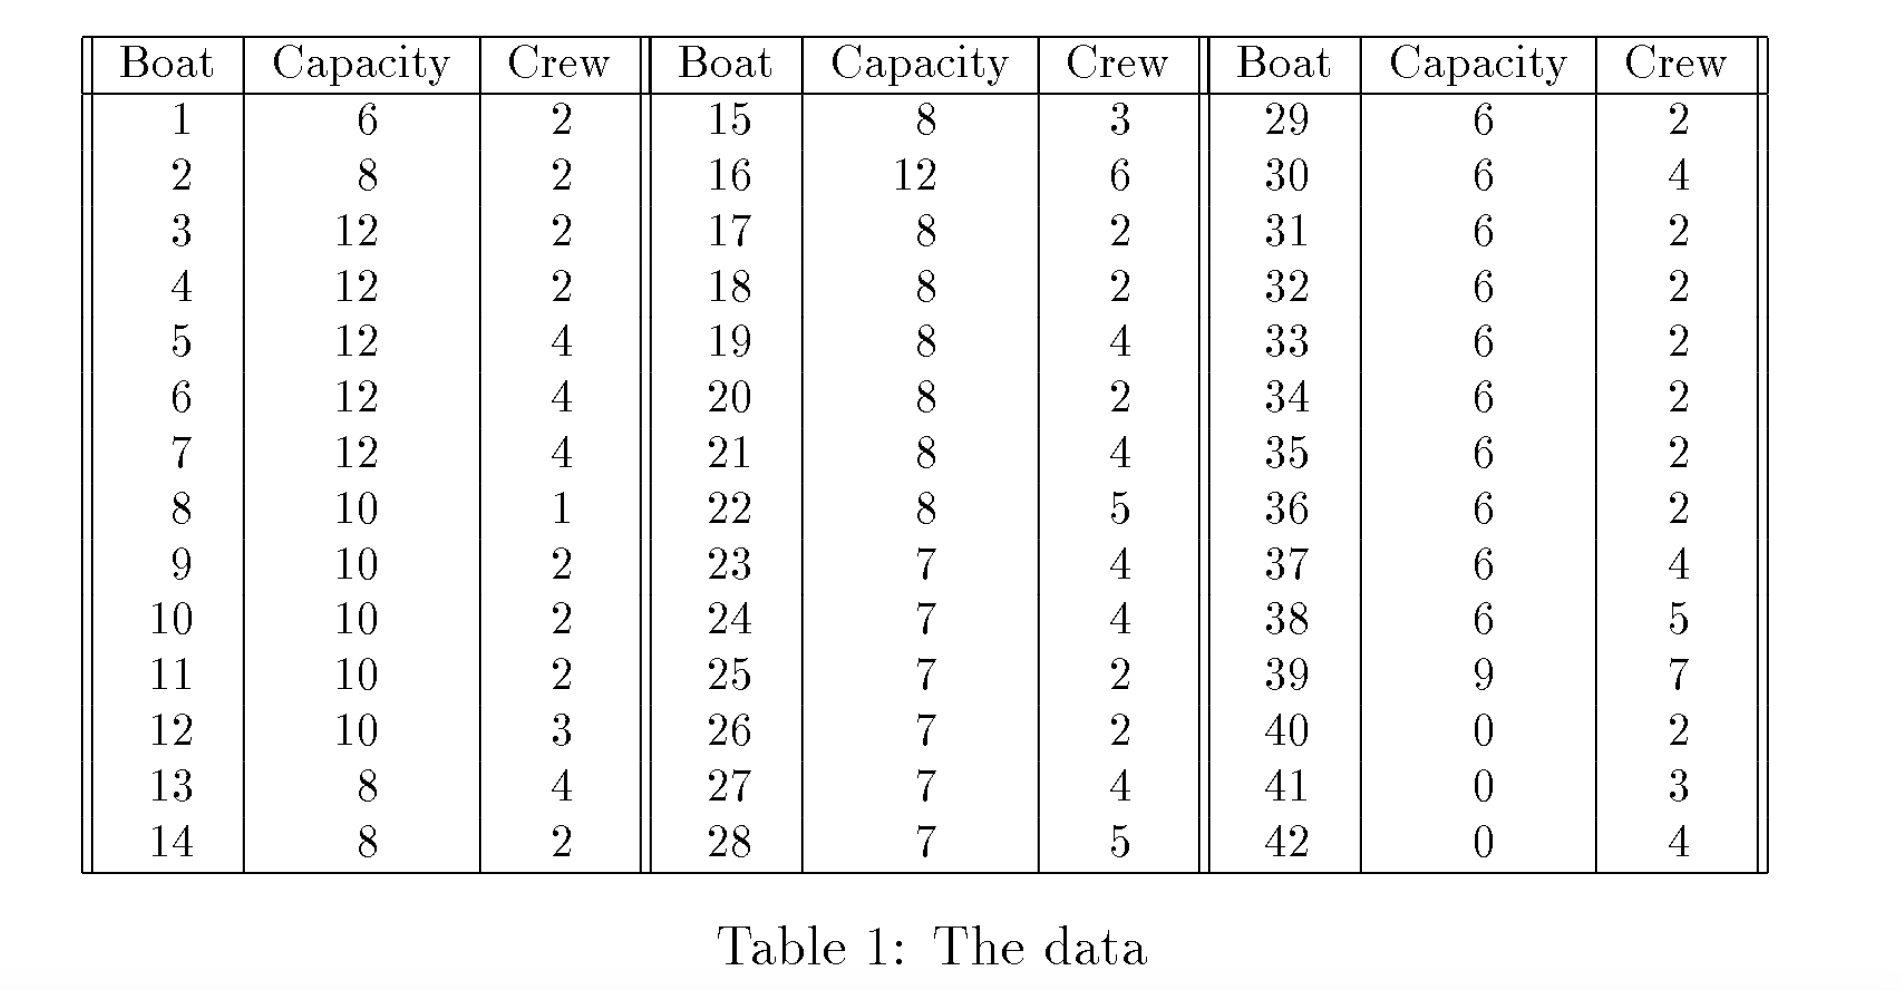
\includegraphics[width=0.7\textwidth]{1}
  \label{fig:DiagramaBarra2}
\end{figure}

\newpage

Por lo tanto identificamos 42 botes (tripulaciones), definimos $\mathit{i},\mathit{j},\mathit{k} \in \{1,..,42\}$ y un conjunto de tiempos $\mathit{t} \in \{1,...,6\}$.

\begin{enumerate}
\item El tamaño de las tripulaciones estara dada por $\mathit{s}_{\mathit{i}}$, y la capacidad del bote - la maxima cantidad de personas que el bote puede recibir incluyendo los dueños del bote es de $\mathit{C}_{\mathit{i}}$.

\item El numero maximo de invitados que puede cada bote invitar es de $\mathit{c}_{\mathit{i}}$ = max (0,$\mathit{C}_{\mathit{i}}$-$\mathit{s}_{\mathit{i}}$).

\item Se introduce la variable binaria $\mathit{x}_{\mathit{i},\mathit{j},\mathit{t}}$. La variable $\mathit{x}_{\mathit{i},\mathit{j},\mathit{t}}$ = 1 si la tripulacion huesped $\mathit{j}$ visita a la tripulacion anfitriona $\mathit{i}$ en el periodo de tiempo $\mathit{t}$. En todo otro caso $\mathit{x}_{\mathit{i},\mathit{j},\mathit{t}}$ = 0.

\item Se utiliza otra variable binaria para decidir cuales botes son anfitriones. La variable $\mathit{h}_{\mathit{i}}$ = 1 si el bote $\mathit{i}$ es anfitrion, en el caso que el bote sea husped $\mathit{h}_{\mathit{i}}$ = 0.

\item Solo hay fiestas en los botes anfitriones, o, si una tripulacion huesped visita a un bote $\mathit{i}$ en algun periodo de tiempo, entonces el bote $\mathit{i}$ es anfitrion.

\item La capacidad maxima de cada bote nunca se puede exceder.

\item No hay tripulaciones hibridas, esto quiere decir que una tripulacion es anfitrion o es huesped.

\item Una tripulacion $\mathit{j}$ visita a otra tripulacion $\mathit{i}$ al menos una vez.

\item Los botes 1,2 y 3 tienen que ser anfitriones. (Barco del organizador y 2 barcos que tenian tripulacion con niños).

\item Los botes 40,41 y 42 deben ser botes huespedes con capacidad 0 (Barco virtual de niños).

\item Las tripulaciones huespedes no pueden encontrarse mas de una vez durante toda la fiesta.

\item Finalmente lo que se busca es minimizar el numero de barcos anfitriones, seleccionar que barcos seran los anfitriones y asignar las tripulaciones huespedes a los barcos anfitriones durante todo lo que dure la fiesta.

\end{enumerate}

El problema en su estructura a permanecido igual durante todos estos años, las variaciones que se proponen son simplemente relajaciones del problema original.

\subsubsection*{The Uncapacitated Problem[ref]}

 La primera variante que se intento resolver de Progressive Party Problem fue resolver el problema sin considerar la capacidad de los barcos, esto quiere decir que un barco puede almacenar a todos las tripulaciones huespedes en un solo periodo. Ahora si pensamos en más de un periodo, es facil ver una cota inferior de barcos anfitriones que necesitaremos para la fiesta, si $\mathit{g}$ tripulaciones huespedes visitan el barco anfitrion $\mathit{i}$ en el periodo 1, necesitaremos al menos $\mathit{g}$ barcos anfitriones en el periodo 2 (Esto es debido a que no podemos volver a visitar el barco $\mathit{i}$ y ademas las tripulaciones huespedes no pueden volver a encontrarse). Por lo tanto necesitaremos $\mathit{g}$ +1 barcos anfitriones para que las tripulaciones de el periodo 1 no se encuentren en el periodo 2, entonces claramente $\mathit{g}$($\mathit{g}$+1) es la cantidad maxima de tripulacion huesped que podemos acomodar en los 2 periodos utilizando solo g+1 barcos anfitriones. Usando lo anterior, para una instancia de 6 anfitriones podemos acomodar 30 huespedes, para una instancia de 7 anfitriones podemos acomodar 42 huespedes. Para el caso en particular de 42 botes en total, 7 seran anfitriones( 35 huespedes). Ahora como en la vida real los barcos tienen una capacidad maxima, por lo tanto este enfoque no es el mas indicado.
 
 \newpage
 
\subsubsection*{A Lower Bound[ref]}

Considerar la capacidad de los barcos es muy importante si es que se quiere encontrar una solucion aceptable para este problema, es por esto que se busco otro enfoque. La segunda variante propuesta del problema, tambien una relajacion, es resolver el problema considerando que no existen distintas tripulaciones huespedes, si no que existe una unica y gigante tripulacion huesped. Lo que se busca con esto es encontrar cual es la cantidad de botes anfitriones que se necesitan para que quepan toda la tripulacion huesped en el primer periodo. Lo que no se esta considerando aca es que los miembros de cada  tripulacion deban permanecer juntos.
 
\subsubsection*{Otras Variantes}

Otra variante del problema es resolver el problema como un CSP, es decir, encontrar una instanciación de las variables que cumpla las restricciones sin una función objetivo. Finalmente la ultima variante que nombraremos sera cambiar la función objetivo de tal manera de maximizar la cantidad de periodos, con el fin de que la fiesta dure mas.

\section*{Estado del Arte}

Como el problema data del año 1996, muchos autores han propuesto estrategias y algoritmos para resolver el Progressive Party Problem, algunos de estos metodos utilizados los presentaremos en esta sección

\begin{itemize}
\item Los primeros metodos se comenzaron a proponer en 1996, el mismo autor del problema, Peter Hubbard y su equipo comenzaron a resolver dos variantes del problema del Progressive Party Problem, estas fueron las variantes The Uncapacitated Problem y  Total Crew Progressive Party Problem. El fin de resolver estos dos problemas fue para encontrar una cota inferior sobre la cantidad de botes anfitriones que se necesitarian para cierta cantidad de tripulaciones huespedes.
Luego de haber resuelto los dos problemas anterior, Peter y su equipo hicieron dos formulaciones usando programacion lineal entera con el fin de resolver el problema. 

La primera formulación se utilizaron variables binarias para resolver un CSOP con el objetivo de minimizar la cantidad de barcos anfitriones, el numero de restricciones de este modelamiento fue del orden de O($B^{4}T^{2}$), donde B es el numero de botes y T la cantidad de periodos, el numero variables fue moderado, alrededor de O($B^{2}T$). Se corrieron pruebas utilizando 14 botes y 4 periodos de tiempo, el modelo resulto tener 379 variables y 18212 filas, el resultado fue obtenido despues de 259 segundos utilizando XPRESSMO optimiser[ref] en una IBM 486 DX PC, en tan solo 816 iteraciones.

La segunda formulación tambien se utilizo variables binarias, se hicieron algunos cambios en las restricciones, el objetivo de esta formulación fue el reducir la cantidad de restricciones, lograndose bajar a O($B^{3}T$) pero con el costo de que aumentaron el numero de variables a O($B^{3}T$). Las mismas pruebas que se realizaron en la primera formulación se utilizaron con este segundo modelo, obteniendo los mismos resultados pero en un tiempo menor.

Finalmente cuando se intento resolver el problema completo utilizando las dos formulaciones anteriores, se fallo con ambas modelos. Debido a lo anterior se decidio relajar el problema, fijando que el minimo numero de barcos anfitriones deberian estar entre 13 y 15 (Esto se baso en los resultados obtenidos de las cotas inferiores obtenidas en los problemas the Uncapacitated Problem y  Total Crew Progressive Party Problem), ademas se ignoro la restriccion de que las tripulaciones huespedes se puedan encontrar mas de una vez, la solución fue encontrada en 598 segundos. Al ver que esta euristica funcionaba, la de fijar un rango en la cantidad de botes anfritriones, se corrio un segun intento, que fallo al no arrojar ningun resultado luego de 189 horas.

Luego de que los modelos de programación lineal fallaran, el equipo modelo el Progressive Party Problem como un CSP, se logra eliminar la función objetivo ya que previamente se definen quienes seran los 13 barcos anfitriones, se eliguen 13 debido a la cota inferios que se encontro previamente cuando se penso en una gran tripulación huesped. Este CSP fue resuelto usando una libreria de C++ llamada ILOG Solver, la libreria posee una implementacion de backtracking con full lookahead. La ventaja que tiene este modelo de estilo CSP es la cantidad de variables y restricciones que estas tienen, ambas estan alrededor de O($B^{2}T$). Finalmente se logro encontrar una resultado utilizando 13 botes anfitriones, 29 huespedes y 6 periodos en 27 minutos, tambien arrojo buenos resultados con 7 y 8 periodos.

\begin{figure}[!h]
  \centering
    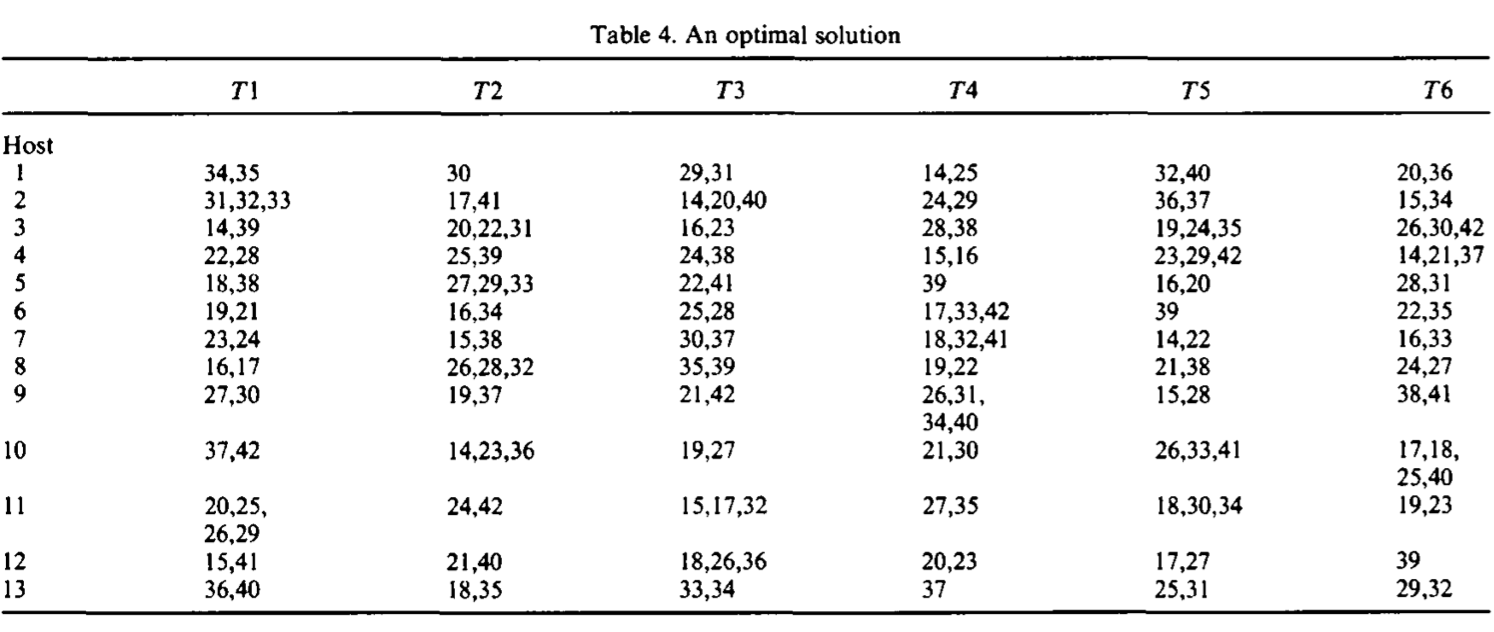
\includegraphics[width=0.9\textwidth]{2}
    \caption{Ejemplo de solución optima}
  \label{fig:DiagramaBarra3}
\end{figure}


\item En 1997, Joachim P. Walser fue uno de los pioneros en utilizar algorimos de busqueda local para resolver este problema, el algoritmo que lleva por nombre WSAT, realiza una busqueda local usando Greedy con restricciones pseudo-booleanas , ademas viene con un mecanismo de historial y una lista taboo. Este algoritmo trabaja dentro del mundo de lo factible, se define un movimiento, y cada vez que se realiza este se va calculando un score, si este score disminuye nos vamos quedando con la nueva instanciación, cuando el score llega a 0 quiere decir que estamos en presencia de la solución optima.  En caso de que exista un empate entre score, se utiliza la lista historia para regresar a la instanciación mas antigua, obviamente ignorando las instanciaciones que se encuentran en la lista taboo. Para resolver el Progressive Party Problem, Walser se baso en el trabajo hecho por Peter Hubbard y su equipo, utilizo el mismo modelo CSP, utilizo los 13 botes propuestos por Peter Hubbard y ademas genero 5 instanciaciones de los 13 botes iniciales considerados como anfitriones(Asegurandose que la capacidad de los 13 botes sean suficente para las tripulacion huesped), ademas se modificaron ciertas restricciones del CSP original a restricciones del tipo Pseudo-Boleanas y finalmente, se fijo el tamaño de la lista tabu en 1. Se obtuvieron los siguientes resultados.

\newpage 

\begin{figure}[!h]
  \centering
    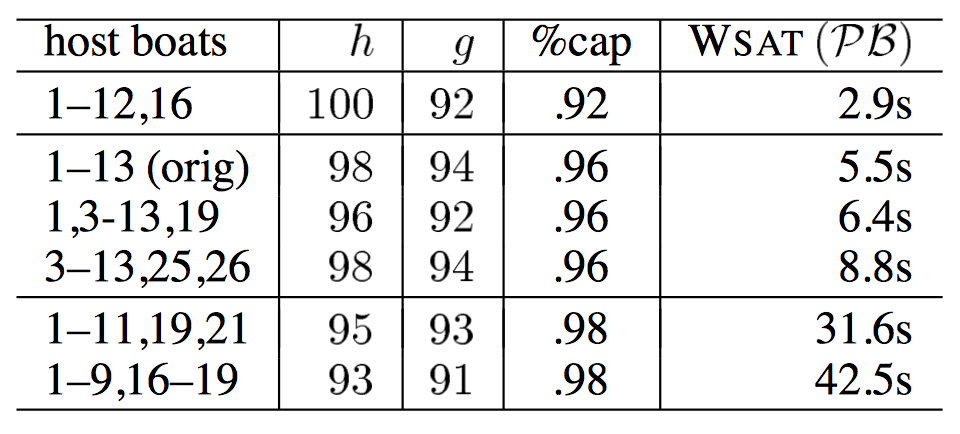
\includegraphics[width=0.4\textwidth]{3}
  \label{fig:DiagramaBarra4}
\end{figure}

La tabla anterior muestra los botes anfitriones seleccionados, la capacidad maxima de los botes, la cantidad total de huespedes, porcentaje total de la capacidad utilizada y tiempo promedio de correr el algoritmo 20 veces, los resultados fueron considerablemente mas bajo que el modelo propuesto por el trabajo de  Peter Hubbard. Adicionalmente se resolvio el CSP original utilizando Oz, un lenguaje de restriccion concurrente, con el fin de comparar con el Solver ILOG que se utilizo incialmente para resolver el problema, el tiempo que demoro Oz fue de 8 minutos, en una maquina conocida como SPARCstation 20, en cambio, el Solver ILOG demoro 27 minutos, tambien se aprecia una disminución notable en el tiempo de resolución del problema.

\item En 1999 Philippe Galinier junto a Jin-Kao Hao propusieron una tercera forma de resolver este problema, su metodo de resolución se basa en busqueda local, trabajando en el mundo de lo infactible resolviendo el CSP propuesto por Peter Hubbard y su equipo. Para resolver el Progresive Parting Problem, ellos introducen un espacio de busqueda, una función de costo y dos diferentes vecindarios, donde se experimentan con ambos utilizando distintas heuristicas. El espacio de busqueda que ellos utilizan es de de G x T, donde G es igual a 29 y T $\in$ (6,7,8,9,10), este espacio de busqueda se justifica dado que el CSP ya estan asignados los 13 barcos anfitriones, por lo tanto debemos  asignar las 29 tripulaciones en los t periodos que definamos. La función de costo que proponen es una función que castiga cada restricción incumplida, castigando mas a las restricciones duras que las blandas.Los dos vecindarios que generan dependen de los dos movimientos que ellos proponen, el primer movimiento corresponde a cambiar el barco anfitrion de una tripulación huesped con conflicto, esto quiere decir que se iran probando distintos barcos anfitriones quedandose con el barco anfitrion que presente menos conflictos. El segundo movmiento correponde a hacer un swap entre los barcos anfitriones asignados a dos tripulaciones huespedes. Ya definido lo anterior, Galinier y Hao utilizan dos algorimos para resolver el problema, uno de ellos es tabu search[ref] y el segundo es conocido como metropolis (Version simplificada de Simulated Annealing[ref]). Finalmente se definem cuatro criterios de parada

\begin{enumerate}
	\item Si la función de costo es igual a 0.
	\item Si se alcanza el tiempo maximo establecido para que el algoritmo se ejecute.
	\item Si se alcanza el maximo numero de iteraciones.
	\item Si se alcanza el maximo numero de movimientos.
\end{enumerate}

La implementación fue realizaca en C++ y ejecutada en una maquina conocida como Sun ULTRA 1. Los resultados se muestra en una tabla donde se compara el tiempo que demora en encontrar una solución utilizando ILP(Integer Linear Programing) y la resolución del CSP propuestos por Peter Hubbard vs los algoritmos de busqueda local propuestos.

\newpage


\begin{table}[h!]
\centering
   \begin{tabular}{|l|l|l|l|}
    \hline
    Problem & ILP  & Publisher CSP resolution & LS     \\ \hline
    p6      & fail & 27 min                   & $<$ 1 s. \\
    p7      & fail & 28 min                   & $<$1 s. \\
    p8      & fail & fail                     & 1 s.   \\
    p9      & fail & fail                     & 4 s.   \\
    p10     & fail & fail                     & fail   \\ \hline
    \end{tabular}
\end{table}

Se corrieron los experimentos 20 veces, el tiempo promedio obtenido por los algoritmos de busqueda local son muchos mas bajos que los resueltos por ILOG Solver. Si bienlos algoritmos  pudieron resolver para 6,7,8 y 9 periodos, observamos que para 10 periodos el algoritmo falla en resolver el problema. Para finalizar observemos la siguiente tabla del costo entregado al intentar resolver el problema con 9 periodos de tiempo utilizando los algoritmos de  busqueda local.

\begin{figure}[!h]
  \centering
    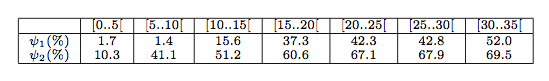
\includegraphics[width=0.8\textwidth]{4}
  \label{fig:DiagramaBarra5}
\end{figure}

La tabla indica en cada columa el porcentaje de soluciones que tuvieron un costo dentro de ese intervalo, es decir, en la columna nos dice que el 1.7$\%$ de los resultados obtenidos obtuvieron un costo de 0,1,2,3 o 4. Esta información es importante ya que nos permite comparar y observar que el segundo movimiento fue mucho mas efectivo que el primer movimiento.

\item 2 papers mas ? 


\end{itemize}

\bibliographystyle{plain}
\bibliography{Referencias}


\end{document} 